\documentclass[11pt]{article}

% Increase main memory size
\usepackage{etex}
\usepackage{morewrites}
\usepackage{multicol}
\usepackage{pgfplots}
\usepackage{tikz}
\usetikzlibrary{external}
\tikzexternalize[prefix=cached_models/]

\usepackage{etex}
\usepackage{morewrites}
\usepackage{enumitem}
\usepackage{float}
\usepackage[linesnumbered,ruled,vlined]{algorithm2e}
\usepackage{algorithmicx}
\usepackage{algpseudocode}

% Define \Comment for algorithmicx
\renewcommand{\Comment}[1]{\hfill\textit{// #1}}
\listfiles

\usepackage{amsmath, amssymb, amsthm}
\usepackage{graphicx}
\usepackage{geometry}
\usepackage{array}
\usepackage{booktabs}
\usepackage{float}
\usepackage{verbatim}
\usetikzlibrary{3d}

% Page Layout
\geometry{a4paper, margin=1in}
\setlength\parindent{0pt}
\pgfplotsset{compat=1.18}

% Custom commands
\newcommand{\card}[1]{\lvert #1 \rvert}
\newcommand{\inner}[2]{\left\langle #1, #2 \right\rangle}

\title{\textbf{Numerical Linear Algebra}}
\author{}
\date{}

\begin{document}

\maketitle

\section{Matrices, Vectors, and Norms}
\subsection{Matrix-Vector Multiplication}
Given a matrix \( A \in \mathbb{C}^{m \times n} \) and a vector \( x \in \mathbb{C}^n \), the matrix-vector product \( Ax = b \in \mathbb{C}^m \) is defined as:

\[
b_i = \sum_{j=1}^{n} a_{ij} x_j, \quad \text{for } i = 1, \ldots, m
\]

where \( a_{ij} \) are the entries of the matrix \( A \).

\subsubsection*{Observation}
The transformation \( x \mapsto Ax \) is a linear transformation from \( \mathbb{C}^n \) to \( \mathbb{C}^m \), i.e., it satisfies:
\[
A(x + y) = Ax + Ay, \quad A(\alpha x) = \alpha Ax, \quad \text{for all } x, y \in \mathbb{C}^n, \alpha \in \mathbb{C}
\]

\subsubsection{A Matrix times a Vector}
\[b = Ax = \sum_{j=1}^{n} x_j a_j\]
where \( a_j \) is the \( j \)-th column of \( A \).

\[\begin{bmatrix}
b_1 \\
b_2 \\
\vdots \\
b_m
\end{bmatrix} =
\begin{bmatrix}
a_{11} & a_{12} & \cdots & a_{1n} \\
a_{21} & a_{22} & \cdots & a_{2n} \\
\vdots & \vdots & \ddots & \vdots \\
a_{m1} & a_{m2} & \cdots & a_{mn}
\end{bmatrix}
\begin{bmatrix}
x_1 \\
x_2 \\
\vdots \\
x_n
\end{bmatrix} =
x_1
\begin{bmatrix}
a_{11} \\
a_{21} \\
\vdots \\
a_{m1}
\end{bmatrix} +
x_2
\begin{bmatrix}
a_{12} \\
a_{22} \\
\vdots \\
a_{m2}
\end{bmatrix} + \cdots +
x_n
\begin{bmatrix}
a_{1n} \\
a_{2n} \\
\vdots \\
a_{mn}
\end{bmatrix}\]

\subsubsection*{Example: Vandermonde Matrix}
A Vandermonde matrix is defined as:
\[
A = \begin{bmatrix}
1 & x_1 & x_1^2 & \cdots & x_1^{n-1} \\
1 & x_2 & x_2^2 & \cdots & x_2^{n-1} \\
\vdots & \vdots & \vdots & \ddots & \vdots \\
1 & x_m & x_m^2 & \cdots & x_m^{n-1}
\end{bmatrix} \in \mathbb{C}^{m \times n}
\]

\subsubsection*{Observation}
Let fix the sequence \( \{x_1, x_2, \ldots, x_m \} \). If $p$ and $q$ are polynomials of degree at most $n-1$ and $\alpha$ is a scalar, then:
\begin{enumerate}
    \item $(p + q)$ is a polynomial of degree at most $n-1$, and so are $\alpha p, \alpha q$.
    \item $(p + q)(x_i) = p(x_i) + q(x_i)$ for $i = 1, \ldots, m$.
    \item $(\alpha p)(x_i) = \alpha p(x_i)$ for $i = 1, \ldots, m$.
\end{enumerate}

\subsubsection*{Observation}
Suppose we have a vector \( c \in \mathbb{C}^n \) representing the coefficients of a polynomial \( p(x) = c_0 + c_1 x + c_2 x^2 + \cdots + c_{n-1} x^{n-1} \). Then 
\[p(x_i) = (Ac)_i = c_0 + c_1 x_i + c_2 x_i^2 + \cdots + c_{n-1} x_i^{n-1}\]

Any polynomial of degree at most \( n-1 \) can be represented as
\[p(x) = \begin{bmatrix}
1 & x & x^2 & \cdots & x^{n-1}
\end{bmatrix}
\begin{bmatrix}
c_0 \\
c_1 \\
c_2 \\
\vdots \\
c_{n-1}
\end{bmatrix}
\]

\subsection{Matrix-Matrix Multiplication}
Given matrices \( A \in \mathbb{C}^{l \times m} \) and \( C \in \mathbb{C}^{m \times n} \), the matrix-matrix product \( B = AC \in \mathbb{C}^{l \times n} \) is defined as:

\[
b_{ij} = \sum_{k=1}^{m} a_{ik} c_{kj}, \quad \text{for } i = 1, \ldots, l, j = 1, \ldots, n
\]

So,
\[B = \begin{bmatrix}
b_1 & b_2 & \cdots & b_n
\end{bmatrix} = \begin{bmatrix}
a_1 & a_2 & \cdots & a_m
\end{bmatrix} \begin{bmatrix}
c_1 & c_2 & \cdots & c_n
\end{bmatrix}\]
\[b_j = Ac_j = \sum_{k=1}^{m} c_{kj} a_k, \quad j = 1, \ldots, n\]

\subsubsection*{Example: Outer Product}
Given two vectors \( u \in \mathbb{C}^{m\times 1} \) and \( v \in \mathbb{C}^{1\times n} \), the outer product \( uv^T \in \mathbb{C}^{m \times n} \) is defined as:
\[\begin{bmatrix}
    u_1 \\
    u_2 \\
    \vdots \\
    u_m
\end{bmatrix}
\begin{bmatrix}
    v_1 & v_2 & \cdots & v_n
\end{bmatrix} = \begin{bmatrix}
    u_1 v_1 & u_1 v_2 & \cdots & u_1 v_n \\
    u_2 v_1 & u_2 v_2 & \cdots & u_2 v_n \\
    \vdots & \vdots & \ddots & \vdots \\
    u_m v_1 & u_m v_2 & \cdots & u_m v_n
\end{bmatrix}
\]

\subsubsection*{Example}
Let \( B \in \mathbb{C}^{m \times n} \), let \( a_1, a_2, \ldots, a_n \) be the columns of \( A \in \mathbb{C}^{m \times n} \) and let \( R \in \mathbb{C}^{n \times n} \) be an upper triangular matrix with all its superdiagonal entries equal to 1 such that
\[B = \begin{bmatrix}
    b_1 & b_2 & \dots & b_n
\end{bmatrix} = \begin{bmatrix}
    a_1 & a_2 & \dots & a_n
\end{bmatrix} \begin{bmatrix}
    1 & 1 & \dots & 1 \\
    0 & 1 & \dots & 1 \\
    \vdots & \vdots & \ddots & \vdots \\
    0 & 0 & \dots & 1
\end{bmatrix}\]
Then,
\[b_j = A r_j = \sum_{k=1}^{j} a_k, \quad j = 1, \ldots, n\] 
which is known as the indefinite integral operation.

\subsection{Range and Null Space}
\subsubsection*{Theorem}
The range of a matrix \( A \in \mathbb{C}^{m \times n} \) is the space spanned by its columns, i.e. it's column space.
\begin{quotation}
    \textit{"The set of vectors that can be written as \( Ax \) for some \( x \in \mathbb{C}^n \)."}
\end{quotation}

\subsubsection{Null Space and Rank}
The null space of a matrix \( A \in \mathbb{C}^{m \times n} \) is defined as:
\[\text{span} \{x \in \mathbb{C}^n : Ax = 0\}\]

The rank of a matrix \( A \in \mathbb{C}^{m \times n} \) is defined as the dimension of its range:
\[\text{rank}(A) = \dim(\text{range}(A))\]

\subsubsection*{Theorem}
For any matrix \( A \in \mathbb{C}^{m \times n}, m \geq n \), \( A \) has full rank if and only if it maps no two distinct vectors to the same vector:
\[Ax = Ay \implies x = y, \forall x, y \in \mathbb{C}^n \quad \text{and} \quad Ax \neq Ay \implies x \neq y, \forall x, y \in \mathbb{C}^n\]

\subsubsection{Non-singular Matrices}
A non-singular matrix, or invertible matrix is a square matrix \( A \in \mathbb{C}^{n \times n} \) that has full rank.

\subsubsection{Inverse of a Matrix}
The matrix \( A \in \mathbb{C}^{n \times n} \) is the inverse of \( Z \) if and only if:
\[AZ = ZA = I = \begin{bmatrix}
    e_1 & e_2 & \cdots & e_n
\end{bmatrix}\]
where \( e_i \) is the \( i \)-th standard basis vector. Furthermore, the inverse of a matrix is unique and
\[\text{rank}(A) = n = \text{rank}(Z)\]

\subsubsection*{Theorem}
For $A \in \mathbb{C}^{n \times n}$, the following statements are equivalent:
\begin{enumerate}
    \item $A$ has an inverse $A^{-1}$.
    \item $A$ has full rank, i.e. $\text{rank}(A) = n$.
    \item The columns of $A$ span $\mathbb{C}^n$, i.e. $\text{range}(A) = \mathbb{C}^n$.
    \item The columns of $A$ are linearly independent, i.e. $\text{null}(A) = \{0\}$.
    \item $0$ is not an eigenvalue of $A$.
    \item $0$ is not a singular value of $A$.
    \item $\card{A} \neq 0$.
\end{enumerate}

\subsection{Orthogonal Vectors and Matrices}
\subsubsection{Complex Conjugate and Conjugate Transpose}
Given $z \in \mathbb{C}$, the complex conjugate of $z$ is denoted by $\bar{z}$ or $z^*$, where if $z = x + iy$, then $\bar{z} = x - iy$.

The conjugate transpose of a matrix $A \in \mathbb{C}^{m \times n}$ is denoted by $A^*$, where $A^* = \bar{A}^T$.
\[A = \begin{bmatrix}
    a_{11} & a_{12} \\
    a_{21} & a_{22} \\
    a_{31} & a_{32} \\
\end{bmatrix} \implies A^* = \begin{bmatrix}
    \bar{a}_{11} & \bar{a}_{21} & \bar{a}_{31} \\
    \bar{a}_{12} & \bar{a}_{22} & \bar{a}_{32} \\
\end{bmatrix}\]

\subsubsection{Hermitian Matrices and Skew-Hermitian Matrices}
A matrix $A \in \mathbb{C}^{n \times n}$ is called Hermitian if $A^* = A$. (Or $A = A^T$ if $A \in \mathbb{R}^{n \times n}$.)

A matrix $A \in \mathbb{C}^{n \times n}$ is called Skew-Hermitian if $A^* = -A$. (Or $A = -A^T$ if $A \in \mathbb{R}^{n \times n}$.)

\subsubsection{Inner Product and Norm}
Given two vectors $x, y \in \mathbb{C}^n$, the inner product is defined as:
\[\inner{x}{y} = y^* x = \sum_{i=1}^{n} \bar{y}_i x_i\]

The norm of a vector $x \in \mathbb{C}^n$ is defined as:
\[\|x\| = \sqrt{\inner{x}{x}} = \sqrt{\sum_{i=1}^{n} |x_i|^2}\]

The modulus of a complex number $z \in \mathbb{C}$ is defined as:
\[|z| = \sqrt{z \bar{z}} = \sqrt{x^2 + y^2} \quad \text{where } z = x + iy\]

The angle $\theta$ between two vectors $x, y \in \mathbb{C}^n$ is defined as:
\[\cos(\theta) = \frac{\inner{x}{y}}{\|x\| \|y\|}\]

\subsubsection*{Observation}
The inner product is bilinear, which means:
\begin{enumerate}
    \item $\inner{x_1 + x_2}{y} = \inner{x_1}{y} + \inner{x_2}{y}$
    \item $\inner{x}{y_1 + y_2} = \inner{x}{y_1} + \inner{x}{y_2}$
    \item $\inner{\alpha x}{\beta y} = \alpha \bar{\beta} \inner{x}{y}$ for all $\alpha, \beta \in \mathbb{C}$
\end{enumerate}

For all vectors or matrices $A, B$ of compatible dimensions, we have:
\[(A B)^* = B^* A^*\]

\subsubsection{Orthogonal Vectors}
Two vectors $x, y \in \mathbb{C}^n$ are orthogonal if $\inner{x}{y} = 0$.

\subsubsection*{Observation}
If $x$ and $y$ are orthogonal, then they are perpendicular.

With $x = \{x_1, x_2, \ldots, x_n\}$ and $y = \{y_1, y_2, \ldots, y_n\}$, $x$ and $y$ are orthogonal if and only if:
\[\inner{x_i}{y_j} = 0, \quad \forall i, j = 1, 2, \ldots, n\]

\subsubsection{Orthonormal Vectors}
A set of vectors $\{x_1, x_2, \ldots, x_n\} \subset \mathbb{C}^n$ is orthonormal if:
\[\inner{x_i}{x_j} = 0 \text{ for } i \neq j \quad \text{and} \quad \inner{x_i}{x_i} = \|x_i\|^2 = 1\]

\subsubsection*{Observation}
The vectors in an orthogonal set are linearly independent.

\subsubsection{Orthogonal and Unitary Matrices}
A matrix $Q \in \mathbb{R}^{n \times n}$ is orthogonal if its columns form an orthonormal set, i.e. $Q^T Q = QQ^T = I$.

A matrix $U \in \mathbb{C}^{n \times n}$ is unitary if its columns form an orthonormal set, i.e. $U^* U = UU^* = I$.

\subsubsection*{Observation}
If $U \in \mathbb{C}^{n \times n}$ is unitary, then $U^{-1} = U^*$ and 
\[\begin{bmatrix}
    u_1^* \\
    u_2^* \\
    \vdots \\
    u_n^*
\end{bmatrix} \begin{bmatrix}
    u_1 & u_2 & \cdots & u_n
\end{bmatrix} = \begin{bmatrix}
    1 & 0 & \cdots & 0 \\
    0 & 1 & \cdots & 0 \\
    \vdots & \vdots & \ddots & \vdots \\
    0 & 0 & \cdots & 1
\end{bmatrix}
\] 
which implies that $\inner{u_i}{u_j} = \delta_{ij}$ where $\delta_{ij}$ is the Kronecker delta, i.e. $\delta_{ij} = \begin{cases}
1 & \text{if } i = j \\
0 & \text{if } i \neq j
\end{cases}$.

\section{Vector Spaces}
A vector space $\mathcal{V}$ over a field $\mathbb{F}$ (usually $\mathbb{R}$ or $\mathbb{C}$) is a set of objects called vectors, along with two operations: vector addition and scalar multiplication, satisfying the following axioms for all $u, v, w \in \mathcal{V}$ and $\alpha, \beta \in \mathbb{F}$:
\begin{enumerate}
    \item (Closure under addition) $u + v \in \mathcal{V}$
    \item (Commutativity) $u + v = v + u$
    \item (Associativity) $(u + v) + w = u + (v + w)$
    \item (Existence of additive identity) There exists an element $0 \in \mathcal{V}$ such that $u + 0 = u$
    \item (Existence of additive inverses) For each $u \in \mathcal{V}$, there exists an element $-u \in \mathcal{V}$ such that $u + (-u) = 0$
    \item (Closure under scalar multiplication) $\alpha u \in \mathcal{V}$
    \item (Distributivity of scalar multiplication with respect to vector addition) $\alpha (u + v) = \alpha u + \alpha v$
    \item (Distributivity of scalar multiplication with respect to field addition) $(\alpha + \beta) u = \alpha u + \beta u$
    \item (Associativity of scalar multiplication) $\alpha (\beta u) = (\alpha \beta) u$
    \item (Existence of multiplicative identity) $1 u = u$ where $1$ is the multiplicative identity in $\mathbb{F}$
\end{enumerate}

\subsection{Linear Subspaces}
A subset $\mathcal{W}$ of a vector space $\mathcal{V}$ is a subspace if $\mathcal{W}$ is itself a vector space under the operations of addition and scalar multiplication defined on $\mathcal{V}$:
\begin{enumerate}
    \item (Closure under addition) $u + v \in \mathcal{W}$
    \item (Closure under scalar multiplication) $\alpha u \in \mathcal{W}$
\end{enumerate}

\subsection{Linear Independence}
A set of vectors $\{v_1, v_2, \ldots, v_k\} \subset \mathcal{V}$ is linearly independent if the only solution to
\[\alpha_1 v_1 + \alpha_2 v_2 + \cdots + \alpha_k v_k = 0\]
is $\alpha_1 = \alpha_2 = \cdots = \alpha_k = 0$. If there exists a non-trivial solution, the set is linearly dependent.

\subsection{Basis and Dimension}
A basis of a vector space $\mathcal{V}$ is a set of linearly independent vectors that spans $\mathcal{V}$. The dimension of $\mathcal{V}$, denoted $\dim(\mathcal{V})$, is the number of vectors in any basis of $\mathcal{V}$. 

\subsection{Inner Product and Norms}
An inner product on a vector space $\mathcal{V}$ over $\mathbb{F}$ is a function $\inner{\cdot}{\cdot} : \mathcal{V} \times \mathcal{V} \to \mathbb{F}$. The standard inner product on $\mathbb{C}^n$ is defined as:
\[\inner{x}{y} = y^* x = \sum_{i=1}^{n} \bar{y}_i x_i\]

A norm on a vector space $\mathcal{V}$ is a function $\|\cdot\| : \mathcal{V} \to \mathbb{R}$ satisfying:
\begin{enumerate}
    \item (Non-negativity) $\|v\| \geq 0$
    \item (Definiteness) $\|v\| = 0$ if and only if $v = 0$
    \item (Homogeneity) $\|\alpha v\| = |\alpha| \|v\|$ for all $\alpha \in \mathbb{F}$ and $v \in \mathcal{V}$
    \item (Triangle inequality) $\|u + v\| \leq \|u\| + \|v\|$ for all $u, v \in \mathcal{V}$
\end{enumerate}
The $p$-norm on $\mathbb{C}^n$ is defined as:
\[\|x\|_p = \left( \sum_{i=1}^{n} |x_i|^p \right)^{1/p}\]
for $1 \leq p < \infty$, and the $\infty$-norm is defined as:
\[\|x\|_\infty = \max_{1 \leq i \leq n} |x_i|\]

\begin{center}
    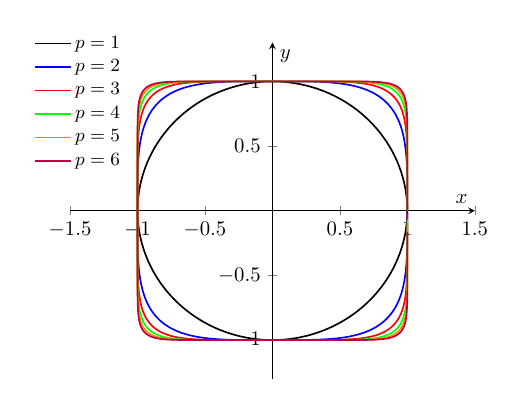
\begin{tikzpicture}[scale=0.75]
        \begin{axis}[
            axis lines = middle,
            xlabel = $x$,
            ylabel = {$y$},
            xmin=-1.5, xmax=1.5,
            ymin=-1.3, ymax=1.3,
            legend style={at={(0.15,0.6)}, anchor=south east, font=\small, draw=none, }
                ]       \addplot [
            domain=0:360, 
            samples=200, 
            smooth, 
            variable=\t, 
            thick,
            black
        ] 
        plot ({cos(\t)}, {sin(\t)});
        \addlegendentry{$p=1$}    
        \addplot [
            domain=0:360, 
            samples=200, 
            smooth, 
            variable=\t, 
            thick,
            blue
        ] 
        plot ({sign(cos(\t))*abs(cos(\t))^(1/2)}, {sign(sin(\t))*abs(sin(\t))^(1/2)});
        \addlegendentry{$p=2$}
        \addplot [
            domain=0:360, 
            samples=200, 
            smooth, 
            variable=\t, 
            thick,
            red
        ] 
        plot ({sign(cos(\t))*abs(cos(\t))^(1/3)}, {sign(sin(\t))*abs(sin(\t))^(1/3)});
        \addlegendentry{$p=3$}
        \addplot [
            domain=0:360, 
            samples=200, 
            smooth, 
            variable=\t, 
            thick,
            green
        ] 
        plot ({sign(cos(\t))*abs(cos(\t))^(1/4)}, {sign(sin(\t))*abs(sin(\t))^(1/4)});
        \addlegendentry{$p=4$}
        \addplot [
            domain=0:360, 
            samples=200, 
            smooth, 
            variable=\t, 
            thick,
            orange
        ] 
        plot ({sign(cos(\t))*abs(cos(\t))^(1/5)}, {sign(sin(\t))*abs(sin(\t))^(1/5)});
        \addlegendentry{$p=5$}
        \addplot [
            domain=0:360, 
            samples=200, 
            smooth, 
            variable=\t, 
            thick,
            purple
        ] 
        plot ({sign(cos(\t))*abs(cos(\t))^(1/6)}, {sign(sin(\t))*abs(sin(\t))^(1/6)});
        \addlegendentry{$p=6$}
        \end{axis}
    \end{tikzpicture}
    \hspace{1cm}
    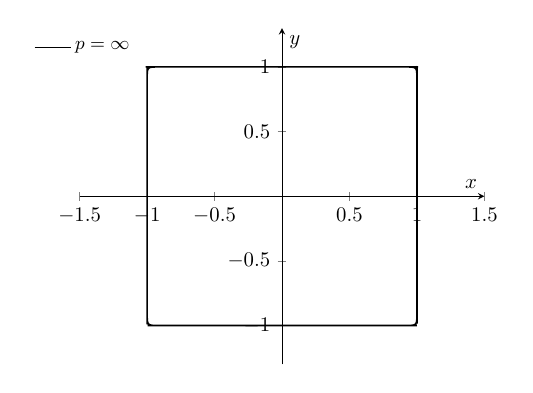
\begin{tikzpicture}[scale=0.75]
        \begin{axis}[
            axis lines = middle,
            xlabel = $x$,
            ylabel = {$y$},
            xmin=-1.5, xmax=1.5,
            ymin=-1.3, ymax=1.3,
            legend pos=north west,
            legend style={font=\small, draw=none, at={(0.15,0.9)}, anchor=south east}
        ]
        \addplot [
            domain=0:500, 
            samples=200, 
            smooth, 
            variable=\t, 
            thick,
            black
        ] 
        ({sign(cos(\t))*abs(cos(\t))^(1/30)}, {sign(sin(\t))*abs(sin(\t))^(1/30)});
        \addlegendentry{$p=\infty$}
        \end{axis} 
    \end{tikzpicture}
\end{center}

\subsubsection{Lemma}
Let $\|\cdot\|_\alpha$ and $\|\cdot\|_\beta$ be two norms on a finite-dimensional vector space $\mathcal{V}$. Then there exist positive constants $c_1$ and $c_2$ such that for all $v \in \mathcal{V}$:
\[c_1 \|v\|_\alpha \leq \|v\|_\beta \leq c_2 \|v\|_\alpha\]

$\|\cdot\|_\alpha$ and $\|\cdot\|_\beta$ are said to be equivalent norms. In $\mathbb{R}^n$:
\[\|x\|_2 \leq \|x\|_1 \leq \sqrt{n} \|x\|_2\]
\[\|x\|_\infty \leq \|x\|_2 \leq \sqrt{n} \|x\|_\infty\]
\[\|x\|_\infty \leq \|x\|_1 \leq n \|x\|_\infty\]

\section{Matrix Norms}
A matrix norm is a function $\|\cdot\| : \mathbb{C}^{m \times n} \to \mathbb{R}$ satisfying:
\begin{enumerate}
    \item (Non-negativity) $\|A\| \geq 0$
    \item (Definiteness) $\|A\| = 0$ if and only if $A = 0$
    \item (Homogeneity) $\|\alpha A\| = |\alpha| \|A\|$ for all $\alpha \in \mathbb{C}$ and $A \in \mathbb{C}^{m \times n}$ 
    \item (Triangle inequality) $\|A + B\| \leq \|A\| + \|B\|$ for all $A, B \in \mathbb{C}^{m \times n}$
    \item (Sub-multiplicativity) $\|AB\| \leq \|A\| \|B\|$ for all $A \in \mathbb{C}^{m \times n}$ and $B \in \mathbb{C}^{n \times p}$
\end{enumerate}

\subsection{Frobenius Norm}
The Frobenius norm of a matrix $A \in \mathbb{C}^{m \times n}$ is defined as:
\[\|A\|_F = \sqrt{\sum_{i=1}^{m} \sum_{j=1}^{n} |a_{ij}|^2} = \sqrt{\text{trace}(A^* A)}\]

\subsection{Induced Norms}
The induced norm (or operator norm) of a matrix $A \in \mathbb{C}^{m \times n}$ is defined as:
\[\|A\| = \sup_{x \neq 0} \frac{\|Ax\|}{\|x\|} = \sup_{\|x\| = 1} \|Ax\|\]  

\subsection{Consistent Norms}
Let $\|\cdot\|_{m \times n}, \|\cdot\|_{n \times p}$ and $\|\cdot\|_{m \times p}$ be three matrix norms on $\mathbb{C}^{m \times n}, \mathbb{C}^{n \times p}$ and $\mathbb{C}^{m \times p}$ respectively. They are said to be consistent if:
\[\|AB\|_{m \times p} \leq \|A\|_{m \times n} \|B\|_{n \times p}, \quad \forall A \in \mathbb{C}^{m \times n}, B \in \mathbb{C}^{n \times p}\]

\subsection{Properties of Induced Norms}
\begin{enumerate}
    \item $\|Ax\| \leq \|A\| \|x\|$ for all $A \in \mathbb{C}^{m \times n}$ and $x \in \mathbb{C}^n$
    \item $\|AB\| \leq \|A\| \|B\|$ for all $A \in \mathbb{C}^{m \times n}$ and $B \in \mathbb{C}^{n \times p}$
    \item $\|A\|_\infty = \max_{1 \leq i \leq m} \sum_{j=1}^{n} |a_{ij}|$ (maximum absolute row sum)
    \item $\|A\|_1 = \max_{1 \leq j \leq n} \sum_{i=1}^{m} |a_{ij}|$ (maximum absolute column sum)
    \item $\|A\|_2 = \sqrt{\lambda_{\max}(A^* A)}$ (with $\lambda_{\max}$ the largest eigenvalue)
    \item $\|A\|_2 = \|A^T\|_2$
    \item $\|A\|_2 = \max |\lambda_i(A)|$ if $A$ is normal (i.e. $A^* A = A A^*$)
    \item $\|A\|_F = \sqrt{\text{trace}(A^* A)}$
\end{enumerate} 

So, in general,
\[\|A\|_\alpha = \max_{x \neq 0} \frac{\|Ax\|_\alpha}{\|x\|_\alpha} = \max_{\|x\|_\alpha = 1} \|Ax\|_\alpha\]

The Frobenius norm is consistent with the euclidean vector norm, but it is not an induced norm.

\subsection{Equivalence of Matrix Norms}
Let $\|\cdot\|_\alpha$ and $\|\cdot\|_\beta$ be two matrix norms on $\mathbb{C}^{m \times n}$. Then there exist positive constants $c_1$ and $c_2$ such that for all $A \in \mathbb{C}^{m \times n}$:
\[c_1 \|A\|_\alpha \leq \|A\|_\beta \leq c_2 \|A\|_\alpha\]

\section{Conditioning and Stability}
\subsection{Conditioning}
The conditioning is a measure of how the output value of a function changes with respect to small changes in the input value.
\[f : X \to Y\]
With a small perturbation in the input \( x \) to \( x + \delta x \), the output changes from \( f(x) \) to \( f(x + \delta x) \). We define
\[\delta f = f(x + \delta x) - f(x)\]

We want to measure how large \( \delta f \) is relative to \( f(x) \) when \( \delta x \) is small relative to \( x \).
\subsubsection{Absolute Condition Number}
The normwise absolute condition number of a function \( f \) at a point \( x \) is defined as:
\[\hat{\kappa}_f(x) = \lim_{\delta x \to 0} \sup_{\|\delta x\| \leq \delta} \frac{\|\delta f\|}{\|\delta x\|} \approx \sup_{\|\delta x\| < \delta} \frac{\|\delta f\|}{\|\delta x\|}\]

If \( f \) is differentiable at \( x \), then
\[\hat{\kappa}_f(x) = \lim_{\delta x \to 0} \sup_{\|\delta x\| \leq \delta} \frac{\|\delta f(x)\|}{\|\delta x\|} = \|J_f(x)\|\]
where \( J_f(x) \) is the Jacobian of \( f \) at \( x \).

\subsubsection{Relative Condition Number}
The normwise relative condition number of a function \( f \) at a point \( x \) is defined as:
\[\kappa_f(x) = \lim_{\delta x \to 0} \sup_{\frac{\|\delta x\|}{\|x\|} \leq \delta} \frac{\|\delta f\| / \|f(x)\|}{\|\delta x\| / \|x\|} \stackrel{f \text{ differentiable}}{=} \frac{\|J_f(x)\| \|x\|}{\|f(x)\|}\]
\subsubsection*{Example}
Let \( f : \mathbb{R} \setminus \{0\} \to \mathbb{R} \) be defined as \( f(x) = \dfrac{1}{x} \). Then \( f'(x) = -\dfrac{1}{x^2} \) and
\[\hat{\kappa}_f(x) = |f'(x)| = \frac{1}{|x|^2}, \quad \kappa_f(x) = \frac{|f'(x)| |x|}{|f(x)|} = 1\]
As \( x \to 0 \), \( \hat{\kappa}_f(x) \to \infty \) but \( \kappa_f(x) = 1 \). This means that \( f(x) = \frac{1}{x} \) is well-conditioned for all \( x \neq 0 \) in the relative sense, but it is ill-conditioned as \( x \to 0 \) in the absolute sense.

\subsubsection*{Example}
Let \( f : \mathbb{R}^2 \to \mathbb{R} \) be defined as \( f(x,y) = x - y \). Then, \( f \) is differentiable and
\[J_f(x,y) = \begin{bmatrix}1 & -1\end{bmatrix}\]
So,
\[\hat{\kappa}_f(x,y) = \|J_f(x,y)\|_2 = \sqrt{2}, \quad \|\kappa_f(x,y)\|_1 = \frac{\|J_f(x,y)\|_1 \|(x,y)\|_1}{|f(x,y)|} = \frac{2(|x| + |y|)}{|x - y|}\]
As \( x \to y \), \( \kappa_f(x,y) \to \infty \). This means that \( f(x,y) = x - y \) is ill-conditioned when \( x \) is close to \( y \).

\subsubsection*{Example}
Let \( f : \mathbb{R}^2 \to \mathbb{R} \) be defined as \( f(x,y) = \dfrac{x}{y} \). Then
\[\|\kappa_f(x,y)\|_2 = \left|\frac{x}{y}\right| + \left|\frac{y}{x}\right|\]
As \( y \to 0 \) or \( x \to 0 \), \( \kappa_f(x,y) \to \infty \). This means that \( f(x,y) = \dfrac{x}{y} \) is ill-conditioned when \( y \) or \( x \) is close to \( 0 \).

\subsection{Stability}
An algorithm is stable if it produces an output that is close to the exact solution of a problem. Formally, an algorithm \( \hat{f} \) for the problem \( f : X \to Y \) is \textbf{numerically stable} if for every input \( x \in X \), there exists \(\hat{x} = x + \delta x \in X\) such that
\[\frac{\|\hat{f}(x) - f(\hat{x})\|}{\|f(x)\|} = O(\epsilon_{\text{mach}}) \quad \text{and} \quad \frac{\|x - \hat{x}\|}{\|x\|} = O(\epsilon_{\text{mach}})\]
where \( \epsilon_{\text{mach}} \) is the machine precision.

An algorithm is \textbf{backward stable} if for every input \( x \in X \), there exists \(\hat{x} = x + \delta x \in X\) such that  
\[\hat{f}(x) = f(\hat{x}) \quad \text{and} \quad \frac{\|x - \hat{x}\|}{\|x\|} = O(\epsilon_{\text{mach}})\]

\subsection{Accuracy}
An algorithm \( \hat{f} \) is said to be \textbf{accurate} if it produces results that are close to the true solution \( f(x) \) for all inputs \( x \in X \). Formally, this means that for every input \( x \in X \), the following holds:
\[\frac{\|\hat{f}(x) - f(\hat{x})\|}{\|f(x)\|} = O(\epsilon_{\text{mach}})\]

\subsubsection*{Observation}
A numerically stable algorithm or a backward stable algorithm is accurate if the problem it solves is well-conditioned.
\[\frac{\|\hat{f}(x) - f(\hat{x})\|}{\|f(x)\|} = \frac{\|f(\hat{x}) + \Delta y - f(x)\|}{\|f(x)\|} \leq \frac{\|f(x + \Delta x) - f(x)\|}{\|f(x)\|} + \frac{\|\Delta y\|}{\|f(x)\|} \cdot \|y\|\]
\[\leq \frac{\|f(x + \Delta x) - f(x)\| / \|f(x)\|}{\|\Delta x\| / \|x\|} \cdot \frac{\|\Delta x\|}{\|x\|} + O(\epsilon_{\text{mach}}) = O(\kappa_f(x) \epsilon_{\text{mach}})\]
where \( \Delta x = \hat{x} - x \) and \( \Delta y = \hat{f}(x) - f(\hat{x}) \).

\section{Solving Linear Systems}
Let 
\[A = \begin{bmatrix}
    2 & 1 & 1 & 0 \\
    4 & 3 & 3 & 1 \\
    8 & 7 & 9 & 5 \\
    6 & 7 & 9 & 8
\end{bmatrix}= L \cdot U = \begin{bmatrix}
    1 \\ 
    2 & 1 \\
    4 & 3 & 1 \\
    3 & 4 & 1 & 1
\end{bmatrix} \cdot \begin{bmatrix}
    2 & 1 & 1 & 0 \\
    & 1 & 1 & 1 \\
    & & 2 & 2 \\
    & & & 2
\end{bmatrix}\]
where \( L \) is a lower triangular matrix and \( U \) is an upper triangular matrix. Now, we define \(x_k\) as the \(k\)-th column of \(A\):
\[x_k = \begin{bmatrix}
    x_{1k} \\
    \vdots \\
    x_{kk} \\
    \vdots \\
    x_{nk}
\end{bmatrix} \longrightarrow L_k \cdot x_k = \begin{bmatrix}
    x_{1k} \\
    \vdots \\
    x_{kk} \\
    0 \\
    \vdots \\
    0
\end{bmatrix} \quad \text{where} \quad L_k = \begin{bmatrix}
    1 & & & & & \\
    & \ddots & & & & \\
    & & 1 & & & \\
    & & -l_{k+1,k} & 1 & & \\
    & & \vdots & & \ddots & \\
    & & -l_{n,k} & & & 1
\end{bmatrix}\]
with \( l_{ik} = \dfrac{x_{ik}}{x_{kk}} \) for \( k < i \leq n \). Thus, we can write
\[L_k = I - l_k e_k^T\]
where \( l_k = \begin{bmatrix}
    0 \\
    \vdots \\
    0 \\
    l_{k+1,k} \\
    \vdots \\
    l_{n,k}
\end{bmatrix} \) and \( e_k = \begin{bmatrix}
    0 \\
    \vdots \\
    1 \\
    \vdots \\
    0
\end{bmatrix} \) (1 at the \(k\)-th position).

Therefore,
\[e_k^T l_k = 0 \quad \text{and} \quad (I - l_k e_k^T)(I + l_k e_k^T) = I \implies L_k^{-1} = I + l_k e_k^T\]

\subsubsection*{Example}
Let \( A = L \cdot U = (L_1^{-1} L_2^{-1} L_3^{-1}) \cdot U \) where
\[A = \begin{bmatrix}
    1 & & & \\
    2 & 1 & & \\
    4 & 3 & 1 & \\
    3 & 4 & 1 & 1
\end{bmatrix} \cdot \begin{bmatrix}
    2 & 1 & 1 & 0 \\
    & 1 & 1 & 1 \\
    & & 2 & 2 \\
    & & & 2
\end{bmatrix}\]
Then,
\[L_1 = \begin{bmatrix}
    1 & & & \\
    -2 & 1 & & \\
    -4 & & 1 & \\
    -3 & & & 1
\end{bmatrix}, \quad L_2 = \begin{bmatrix}
    1 & & & \\
    & 1 & & \\
    & -3 & 1 & \\
    & -4 & & 1
\end{bmatrix}, \quad L_3 = \begin{bmatrix}
    1 & & & \\
    & 1 & & \\
    & & 1 & \\
    & & -1 & 1
\end{bmatrix}\]

Consider \(L_k^{-1} \cdot L_{k+1}^{-1} = (I + l_k e_k^T)(I + l_{k+1} e_{k+1}^T) = I + l_k e_k^T + l_{k+1} e_{k+1}^T\) because \(e_k^T l_{k+1} = 0\). Thus,
\[L_1^{-1} \cdots L_{n-1}^{-1} = L = \begin{bmatrix}
    1 & & & & \\
    l_{21} & 1 & & & \\
    l_{31} & l_{32} & 1 & & \\
    \vdots & \vdots & \vdots & \ddots & \\
    l_{n1} & l_{n2} & l_{n3} & \cdots & 1
\end{bmatrix} \]

\subsection{Forward Elimination}
Consider the Forward Elimination algorithm:
\[\text{Input: } A \in \mathbb{R}^{n \times n}, \bar{b} \in \mathbb{R}^n\]
\[\text{Output: } U \in \mathbb{R}^{n \times n}, \bar{b}^* \in \mathbb{R}^n \text{ such that } L A = U \text{ and } L \bar{b} = \bar{b}^*\]

\begin{algorithm}[H]
\KwIn{$A \in \mathbb{R}^{n \times n}, \bar{b} \in \mathbb{R}^n$}
\KwOut{$U \in \mathbb{R}^{n \times n}, \bar{b}^* \in \mathbb{R}^n$ such that $L A = U$ and $L \bar{b} = \bar{b}^*$}
\For{$k = 1$ \textbf{to} $n-1$}{
    \For{$i = k+1$ \textbf{to} $n$}{
        $l_{ik} = \dfrac{a_{ik}}{a_{kk}}$\;
        \For{$j = k$ \textbf{to} $n$}{
            $a_{ij} = a_{ij} - l_{ik} a_{kj}$\;
        }
        $b_i = b_i - l_{ik} b_k$\;
    }
}
\caption{Forward Elimination}
\end{algorithm}
\vskip 0.5cm
So, the output is
\[L \begin{bmatrix}
    A & \vline & \bar{b} 
\end{bmatrix} = \begin{bmatrix}
    U & \vline & \bar{b}^*
\end{bmatrix}
\]

\subsection{Backward Substitution}
Consider the Backward Substitution algorithm:
\[R \bar{x} = \bar{b}, \quad R = \begin{bmatrix}
    r_{11} & r_{12} & \cdots & r_{1n} \\
    0 & r_{22} & \cdots & r_{2n} \\
    \vdots & \vdots & \ddots & \vdots \\
    0 & 0 & \cdots & r_{nn}
\end{bmatrix}\]
\[r_{nn} x_n = b_n \quad \text{and} \quad r_{n-1, n} x_{n-1} + r_{n-1, n} x_n = b_{n-1}\]

\[ x_n = \frac{b_n}{r_{nn}} \quad \text{and} \quad x_i = \frac{b_i - \sum_{j=i+1}^{n} r_{ij} x_j}{r_{ii}}, \quad i = n-1, n-2, \ldots, 1\]
\begin{algorithm}[H]
\KwIn{$U \in \mathbb{R}^{n \times n}$ (upper triangular), $\bar{b} \in \mathbb{R}^n$}
\KwOut{$\bar{x} \in \mathbb{R}^n$ such that $U \bar{x} = \bar{b}$}
$x_n = \dfrac{b_n}{r_{nn}}$\;
\For{$i = n-1$ \textbf{down to} $1$}{
    $x_i = b_i$\;
    \For{$j = i+1$ \textbf{to} $n$}{
        $x_i = x_i - r_{ij} x_j$\;
    }
    $x_i = \dfrac{x_i}{r_{ii}}$\;
}
\caption{Backward Substitution}
\end{algorithm}

\subsection{Solving Triangular Systems}
With \(D \overline{x} = \bar{b}\), \(D \text{ diagonal } (d_{11}, d_{22}, \ldots, d_{nn}) \in \mathbb{R}^{n\times n}\), we can solve for \(\overline{x}\) as follows:
\[x_i = \frac{b_i}{d_{ii}}, \quad i = 1, 2, \ldots, n\]

With \(U \overline{x} = \bar{b}\), \(L\) upper triangular, we can solve for \(\overline{x}\) using backward substitution:
\[\begin{bmatrix}
    u_{11} & u_{12} & \cdots & u_{1n} \\
    0 & u_{22} & \cdots & u_{2n} \\
    \vdots & \vdots & \ddots & \vdots \\
    0 & 0 & \cdots & u_{nn}
\end{bmatrix} \begin{bmatrix}
    x_1 \\
    x_2 \\
    \vdots \\
    x_n
\end{bmatrix} = \begin{bmatrix}
    b_1 \\
    b_2 \\
    \vdots \\
    b_n
\end{bmatrix}\]
\[u_{nn} x_n = b_n \quad \text{and} \quad u_{n-1,n} x_{n-1} + u_{n-1,n} x_n = b_{n-1}\]
\[ x_n = \frac{b_n}{u_{nn}} \quad \text{and} \quad x_i = \frac{b_i - \sum_{j=i+1}^{n} u_{ij} x_j}{u_{ii}}, \quad i = n-1, n-2, \ldots, 1\]

We can define the algorithm for solving \(U \overline{x} = \bar{b}\) where \(U\) is a upper triangular matrix as follows:

\begin{algorithm}[H]
\KwIn{$U \in \mathbb{R}^{n \times n}$ (upper triangular), $\bar{b} \in \mathbb{R}^n$}
\KwOut{$\bar{x} \in \mathbb{R}^n$ such that $U \bar{x} = \bar{b}$}
$x_n = \dfrac{b_n}{u_{nn}}$\;
\For{$i = n-1$ \textbf{down to} $1$}{
    $x_i = b_i$\;
    \For{$j = i+1$ \textbf{to} $n$}{
        $x_i = x_i - u_{ij} x_j$\;
    }
    $x_i = \dfrac{x_i}{u_{ii}}$\;
}
\caption{Solve Upper Triangular System}
\end{algorithm}
\vskip 0.5cm
The cost of this algorithm is as follows:
\[\textbf{Flops} = \sum_{i=1}^{n-1} \left(1 + 2\sum_{j=i+1}^{n} 1\right) = \cdots = \dfrac{(n-2)n}{2} \sim \mathcal{O}(n^2)\]

\subsection{Gaussian Elimination}
The Gaussian Elimination algorithm can be defined as follows:

\begin{algorithm}[H]
\KwIn{$A \in \mathbb{R}^{n \times n}, \bar{b} \in \mathbb{R}^n$}
\KwOut{$U \in \mathbb{R}^{n \times n}, \bar{b}^* \in \mathbb{R}^n$ such that $L A = U$ and $L \bar{b} = \bar{b}^*$}
\For{$k = 1$ \textbf{to} $n-1$}{
    \For{$i = k+1$ \textbf{to} $n$}{
        $t = \dfrac{a_{ik}}{a_{kk}}$; \tcp{t is a factor}
        \For{$j = k$ \textbf{to} $n$}{
            $a_{ij} = a_{ij} - t a_{kj}$\;
        }
        $b_i = b_i - t b_k$\;
    }
}
\caption{Gaussian Elimination}
\end{algorithm}
\vskip 0.5cm
The cost of this algorithm is as follows:
\[\textbf{Flops} = \mathcal{O}(n^3)\]

\subsection{LU Factorization}
With \(A \in \mathbb{R}^{n \times n}\) non-singular, we can factor \(A\) as \(A = L \cdot U\) where \(L\) is a lower triangular matrix with unit diagonal and \(U\) is an upper triangular matrix:
\[L = I + \sum_{k=1}^{n-1} l_k e_k^T \]

\subsubsection*{Observation}
If an \(n \times n\) matrix \(A\) has an LU factorization, then it is unique. Furthermore, if we relax the condition that \(L\) has a unit diagonal (i.e., normalized), then there are infinitely many LU factorizations of \(A\).

\subsubsection*{Theorem}
If all the leading principal minors of \(A\) are non-zero, i.e., \(\det(A_k) \neq 0\) for \(k = 1, 2, \ldots, n-1\) where \(A_k\) is the \(k \times k\) leading principal submatrix of \(A\), then \(A\) has an LU factorization. In particular, if \(A\) is strictly diagonally dominant or symmetric positive definite, then \(A\) has an LU factorization.

\begin{proof}
We will prove this by induction on \(n\). The base case \(n=1\) is trivial since any non-zero scalar can be factored as \(1 \cdot a_{11}\). A matrix with \(k\) row operations already done can be written as
\[A^{(k)} = \begin{bmatrix}
    a_{11} & a_{12} & \cdots & \cdots & a_{1n} \\
    0 & a_{22}^{(2)} & \cdots & \cdots & a_{2n}^{(2)} \\
    0 & 0 & a_{kk}^{(k)} & \cdots & a_{kn}^{(k)} \\
    \vdots & \vdots & \vdots & \ddots & \vdots \\
    0 & 0 & a_{n2}^{(k)} & \cdots & a_{nn}^{(k)}
\end{bmatrix}\]
where every superindex \((k)\) indicates that \(k\) row operations have been performed. Note that the leading principal submatrix of order \(k\) of \(A^{(k)}\) is the same as that of \(A\). Thus, \(\det(A^{(k)}) = \det(A_k) \neq 0\). 
Hence, the next step is possible.
\end{proof}

\subsubsection*{Theorem}
If an invertible matrix \(A \in \mathbb{R}^{n \times n}\) has an LU factorization, then it is unique.
\begin{proof}
Suppose \(A = L_1 U_1 = L_2 U_2\) where \(L_1, L_2\) are lower triangular with unit diagonal and \(U_1, U_2\) are upper triangular. Then,
\[L_2^{-1} L_1 = U_2 U_1^{-1}\]
The left-hand side is lower triangular with unit diagonal, and the right-hand side is upper triangular. Thus, both sides must be equal to the identity matrix. Therefore, \(L_1 = L_2\) and \(U_1 = U_2\).
\end{proof}

\subsection{Pivoting}
We use pivoting to avoid division by zero or small numbers during the elimination process. There are three types of pivoting:
\begin{enumerate}
    \item Partial row pivoting: We interchange rows to ensure that the pivot element is the largest in its column.
        \[|a_{lk}| = \max_{k \leq i \leq n} |a_{ik}^{(k)}|\]
    \item Partial column pivoting: We interchange columns to ensure that the pivot element is the largest in its row.
        \[|a_{kl}| = \max_{k \leq j \leq n} |a_{kj}^{(k)}|\]
    \item Total pivoting: We interchange both rows and columns to ensure that the pivot element is the largest in the remaining submatrix.
        \[|a_{lm}| = \max_{k \leq i,j \leq n} |a_{ij}^{(k)}|\]
\end{enumerate}
Total pivoting is the most stable but also the most expensive. It yields the complete \(LU\) factorization. The cost of partial pivoting is \(\mathcal{O}(n^2)\), while the cost of total pivoting is \(\mathcal{O}(n^3)\).
\vskip 0.5cm
The \(LU\) factorization with partial pivoting algorithm can be defined as follows:

\begin{algorithm}[H]
\caption{LU Factorization with Partial Pivoting}
\KwIn{$A \in \mathbb{R}^{n \times n}, b \in \mathbb{R}^n$}
\KwOut{$P, L, U$ such that $PA = LU$}
\For{$k = 1$ \textbf{to} $n-1$}{
    $l = \arg\max_{k \leq i \leq n} |a_{ik}^{(k)}|$\;
    Swap rows $k$ and $l$ of $A$ and $b$\;
    \For{$i = k+1$ \textbf{to} $n$}{
        $t = \dfrac{a_{ik}}{a_{kk}}$\;
        \For{$j = k$ \textbf{to} $n$}{
            $a_{ij} = a_{ij} - t a_{kj}$\;
        }
        $b_i = b_i - t b_k$\;
    }
}
\end{algorithm}
\pagebreak
\subsection{The role of L and U in Backward Stability}
Let \(A \in \mathbb{R}^{n \times n}\) be a non-singular matrix with \(LU\) factorization \(A = LU\). Then, 
\[\hat{L} \hat{U} = A + \delta A, \quad \frac{\|\delta A\|}{\|L\| \|U\|} = \mathcal{O}(\varepsilon_{\text{mach}})\]
where \(\hat{L}\) and \(\hat{U}\) are the computed factors of \(A\), and \(\delta A\) is the perturbation in \(A\) due to rounding errors.

Now, let us introduce partial pivoting. Let \(P\) be a permutation matrix such that \(PA = LU\). Then,
\[L = \begin{bmatrix}
    \ddots & & & & \\
    l_{ik} & \ddots & & & \\
    \vdots & \vdots & \ddots & & \\
    l_{nk} & l_{n,k+1} & \cdots & \ddots & \\
    l_{n1} & l_{n2} & \cdots & l_{n,n-1} & 1
\end{bmatrix} \implies \|L\| = \mathcal{O}(1)\]

Thus, the stability of the \(LU\) factorization with partial pivoting depends on \(\|U\|\) relative to \(\|A\|\). This ratio is known as the growth factor:
\[\rho = \frac{\max |u_{ij}|}{\max |a_{ij}|}\]

With \(PA = LU\), we have
\[\hat{L} \hat{U} = PA + \delta A, \quad \frac{\|\delta A\|}{\|P\| \|A\|} = \mathcal{O}(\varepsilon_{\text{mach}}) \implies \frac{\|\delta A\|}{\|A\|} = \mathcal{O}(\rho \varepsilon_{\text{mach}})\]

\subsubsection*{Example}
Let
\[A = \begin{bmatrix}
    1 & & & & 1 \\
    -1 & 1 & & & 1 \\
    -1 & -1 & 1 & & 1 \\
    -1 & -1 & -1 & 1 & 1 \\
    -1 & -1 & -1 & -1 & 1
\end{bmatrix} = L \cdot U = \begin{bmatrix}
    1 & & & & \\
    -1 & 1 & & & \\
    -1 & -1 & 1 & & \\
    -1 & -1 & -1 & 1 & \\
    -1 & -1 & -1 & -1 & 1
\end{bmatrix} \cdot \begin{bmatrix}
    1 & & & & 1 \\
    & 1 & & & 2 \\
    & & 1 & & 4 \\
    & & & 1 & 8 \\
    & & & & 16
\end{bmatrix}\]
Then, \(\rho = 16 = 2^{n-1}\), which is not bounded. Then,
\[\frac{\|\delta A\|}{\|A\|} = \mathcal{O}(2^{n-1} \varepsilon_{\text{mach}})\]

\pagebreak
\section{Least Squares}
To compute the QR factorization of a matrix \(A \in \mathbb{R}^{m \times n}\) with \(m \geq n\), we can use different methods such as Gram-Schmidt, given rotations, or Householder reflections.
The QR factorization decomposes \(A\) into an orthogonal matrix \(Q \in \mathbb{R}^{m \times m}\) and an upper triangular matrix \(R \in \mathbb{R}^{m \times n}\):
\[A = Q R\]
where
\[Q = \begin{bmatrix}
    q_1 & q_2 & \cdots & q_m
\end{bmatrix}, \quad R = \begin{bmatrix}
    r_{11} & r_{12} & \cdots & r_{1n} \\
    0 & r_{22} & \cdots & r_{2n} \\
    \vdots & \vdots & \ddots & \vdots \\
    0 & 0 & \cdots & r_{nn} \\
    0 & 0 & \cdots & 0 \\
    \vdots & \vdots & & \vdots \\
    0 & 0 & \cdots & 0
\end{bmatrix}\]
\subsection{Gram-Schmidt Process}
Given a matrix \(A \in \mathbb{R}^{m \times n}\) with linearly independent columns, the Gram-Schmidt process constructs an orthonormal basis for the column space of \(A\).
\[A = \begin{bmatrix}
    a_1 & a_2 & \cdots & a_n
\end{bmatrix}, \quad \text{span}\{a_1, a_2, \ldots, a_n\} = \text{span}\{q_1, q_2, \ldots, q_n\}\]
The Gram-Schmidt process can be defined as follows:
\begin{align*}
    & v_1 = a_1 & \longrightarrow & & q_1 = \frac{v_1}{\|v_1\|} \\
    & v_2 = a_2 - (a_2^T \cdot q_1) \cdot q_1 & \longrightarrow & & q_2 = \frac{v_2}{\|v_2\|} \\
    & v_3 = a_3 - (a_3^T \cdot q_2) \cdot q_2 - (a_3^T \cdot q_1) \cdot q_1 & \longrightarrow  & & q_3 = \frac{v_3}{\|v_3\|} \\
    & \vdots & & & \\
    & v_n = a_n - \sum_{j=1}^{n-1} (a_n^T \cdot q_j) \cdot q_j & \longrightarrow & & q_n = \frac{v_n}{\|v_n\|}
\end{align*}
The coefficients \(q_k\) satisfy the following:
\[q_i \cdot q_j = \delta_{ij} = \begin{cases}
    1 & i = j \\
    0 & i \neq j
\end{cases}\]
The matrix \(R\) can be constructed as follows:
\[R = \begin{bmatrix}
    r_{11} & r_{12} & \cdots & r_{1n} \\
    0 & r_{22} & \cdots & r_{2n} \\
    \vdots & \vdots & \ddots & \vdots \\
    0 & 0 & \cdots & r_{nn}
\end{bmatrix} = \begin{bmatrix}
    \|v_1\| & q_1^T a_2 & \cdots & q_1^T a_n \\
    0 & \|v_2\| & \cdots & q_2^T a_n \\
    \vdots & \vdots & \ddots & \vdots \\
    0 & 0 & \cdots & \|v_n\|
\end{bmatrix}\]
where
\[r_{ij} = \begin{cases}
    q_i^T a_j & i < j \\
    \|v_i\| & i = j \\
    0 & i > j
\end{cases}\]

With this, we can express \(a_k\) as follows:
\[a_1 = q_1 r_{11} = q_1 \|v_1\|\]
\[a_2 = q_1 r_{12} + q_2 r_{22} = q_1 (q_1^T a_2) + q_2 \\|v_2\|\]
\[a_3 = q_1 r_{13} + q_2 r_{23} + q_3 r_{33} = q_1 (q_1^T a_3) + q_2 (q_2^T a_3) + q_3 \|v_3\|\]
\[\vdots\]
\[a_n = q_1 r_{1n} + q_2 r_{2n} + \cdots + q_n r_{nn} = q_1 (q_1^T a_n) + q_2 (q_2^T a_n) + \cdots + q_n \|v_n\|\]
\vskip 0.5cm
The Gram-Schmidt algorithm can be summarized as follows:

\begin{algorithm}[H]
\KwIn{$A \in \mathbb{R}^{m \times n}$ with linearly independent columns}
\KwOut{$Q \in \mathbb{R}^{m \times n}$ with orthonormal columns, $R \in \mathbb{R}^{n \times n}$ upper triangular}
\For{$k = 1$ \textbf{to} $n$}{
    $v_k = a_k$\;
    \For{$j = 1$ \textbf{to} $k-1$}{
        $r_{jk} = q_j^T a_k$ \;
        $v_k = v_k - r_{jk} q_j$\;
    }
    $r_{kk} = \|v_k\|$\;
    $q_k = \dfrac{v_k}{r_{kk}}$\;
}
\caption{Gram-Schmidt Process}
\end{algorithm}
\vskip 0.5cm
This algorithm can be modified to improve numerical stability, resulting in the Modified Gram-Schmidt algorithm:

\begin{algorithm}[H]
\KwIn{$A \in \mathbb{R}^{m \times n}$ with linearly independent columns}
\KwOut{$Q \in \mathbb{R}^{m \times n}$ with orthonormal columns, $R \in \mathbb{R}^{n \times n}$ upper triangular}
\For{$k = 1$ \textbf{to} $n$}{
    $v_k = a_k$\;
    $r_{kk} = \|v_k\|$\;
    $q_k = \dfrac{v_k}{r_{kk}}$\;
    \For{$j = k+1$ \textbf{to} $n$}{
        $r_{kj} = q_k^T a_j$\;
        $a_j = a_j - r_{kj} q_k$\;
    }
}
\caption{Modified Gram-Schmidt Process}
\end{algorithm}

\subsubsection*{Remark}
The matrix \(R\) is invertible if and only if the columns of \(A\) are linearly independent. The reduced QR factorization is unique up to a sign.

\subsection{Householder Transformations}
A Householder transformation is a linear transformation that reflects a vector about a plane or hyperplane. It is defined as follows:

Given a vector \(v \in \mathbb{R}^n\), the Householder transformation \(H\) is defined as:
\[H = I - 2 \frac{u u^T}{\|u\|}\]
where \(u = v - \alpha e_1\), \(\alpha = \|v\|\), and \(e_1\) is the first standard basis vector in \(\mathbb{R}^n\).  

\end{document}